\documentclass{standalone}
\usepackage{amsmath, amsfonts, amsthm}
\usepackage{graphicx}
\usepackage{tikz}
\usepackage{circuitikz}
\usetikzlibrary{patterns}
\usepackage{scalerel}
\usepackage{pict2e}
\usepackage{tkz-euclide}
\usetikzlibrary{calc}
\usetikzlibrary{arrows.meta}
\usetikzlibrary{shadows}
\usetikzlibrary{external}
\usetikzlibrary{decorations.pathmorphing}
\usetikzlibrary{shapes.geometric}
\usetikzlibrary{arrows,shapes.gates.logic.US,shapes.gates.logic.IEC,calc}
\usepackage{pgfplots}
\pgfplotsset{compat=newest}
\usepgfplotslibrary{statistics}
\usepgfplotslibrary{fillbetween}

\begin{document}
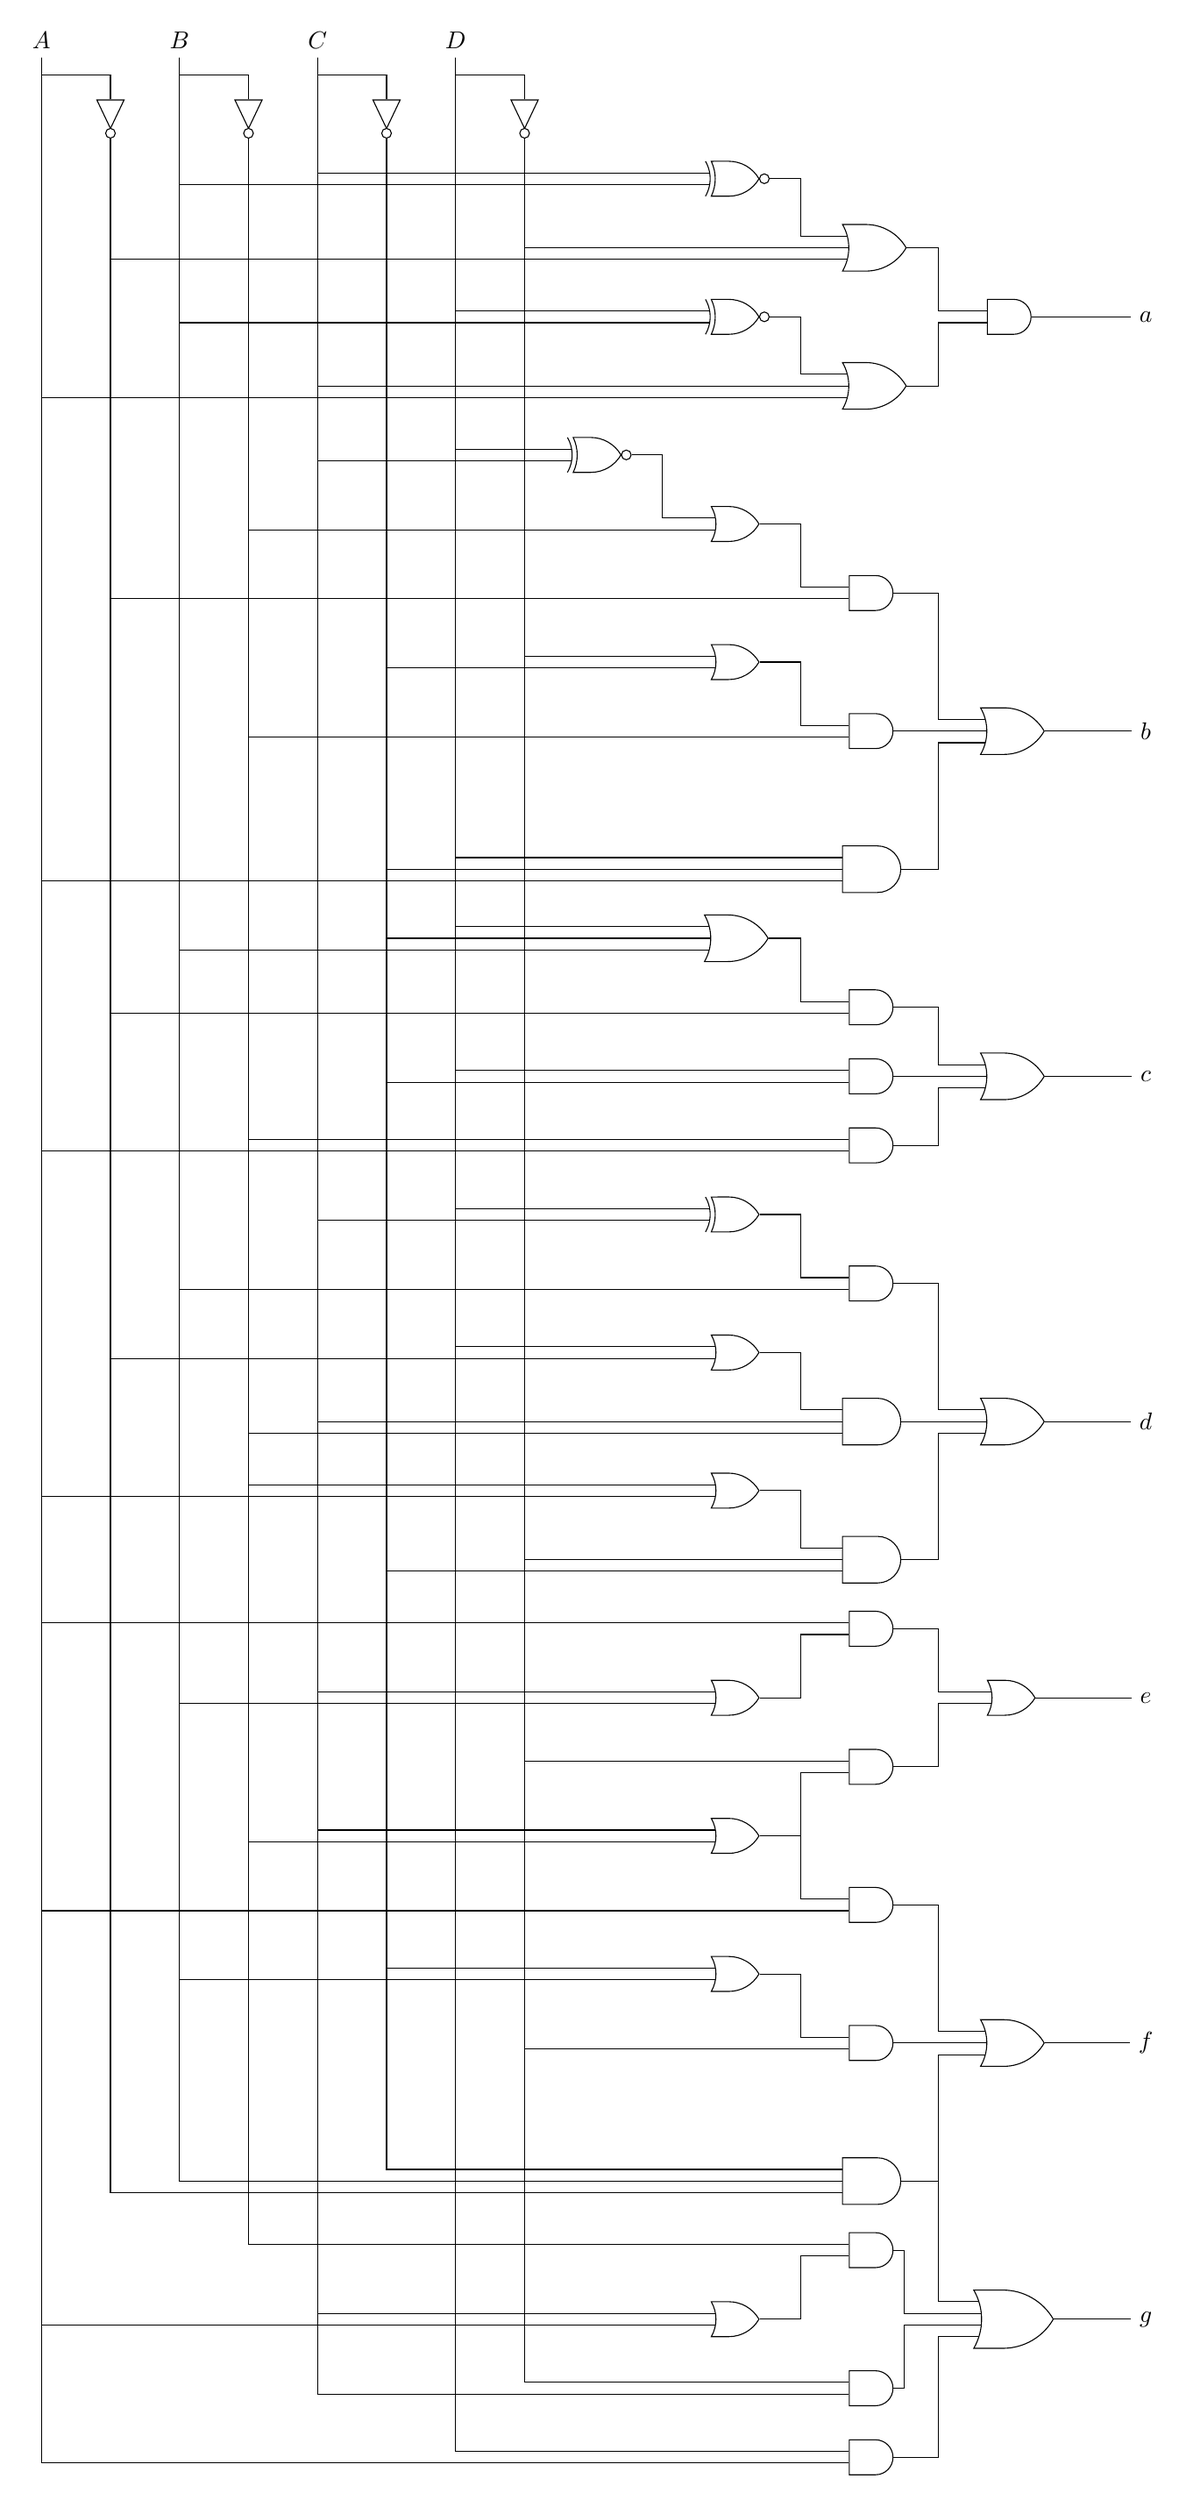
\begin{tikzpicture}
	\node (A) at (-1, 0) {$A$};
	\node (B) at (1, 0) {$B$};
	\node (C) at (3, 0) {$C$};
	\node (D) at (5, 0) {$D$};

	\node[not gate US, draw, rotate=-90] at (0, -1) ('A) {};
	\node[not gate US, draw, rotate=-90] at (2, -1) ('B) {};
	\node[not gate US, draw, rotate=-90] at (4, -1) ('C) {};
	\node[not gate US, draw, rotate=-90] at (6, -1) ('D) {};

	\draw (A) -- (-1, -0.5) -| ('A.input);
	\draw (B) -- (1, -0.5) -| ('B.input);
	\draw (C) -- (3, -0.5) -| ('C.input);
	\draw (D) -- (5, -0.5) -| ('D.input);

	% a

	\node[xnor gate US, draw, logic gate inputs=nn] at (9, -2) (B * C) {};
	\node[xnor gate US, draw, logic gate inputs=nn] at (9, -4) (B * D) {};

	\node[or gate US, draw, logic gate inputs=nnn] at (11, -3) (aOr1) {};
	\node[or gate US, draw, logic gate inputs=nnn] at (11, -5) (aOr2) {};

	\node[and gate US, draw, logic gate inputs=nn] at (13, -4) (aAnd1) {};

	\draw (B) |- (B * C.input 2) {};
	\draw (C) |- (B * C.input 1) {};
	\draw (B) |- (B * D.input 2) {};
	\draw (D) |- (B * D.input 1) {};

	\draw ('A.output) |- (aOr1.input 3) {};
	\draw (B * C.output) -- (10, -2) |- (aOr1.input 1) {};
	\draw ('D.output) |- (aOr1.input 2) {};

	\draw (A) |- (aOr2.input 3) {};
	\draw (B * D.output) -- (10, -4) |- (aOr2.input 1) {};
	\draw (C) |- (aOr2.input 2) {};

	\draw (aOr1.output) -- (12, -3) |- (aAnd1.input 1) {};
	\draw (aOr2.output) -- (12, -5) |- (aAnd1.input 2) {};

	% b

	\node[xnor gate US, draw, logic gate inputs=nn] at (7, -6) (C * D) {};
	\node[or gate US, draw, logic gate inputs=nn] at (9, -7) (bOr1) {};
	\node[or gate US, draw, logic gate inputs=nn] at (9, -9) (bOr2) {};
	\node[and gate US, draw, logic gate inputs=nn] at (11, -8) (bAnd1) {};
	\node[and gate US, draw, logic gate inputs=nn] at (11, -10) (bAnd2) {};
	\node[and gate US, draw, logic gate inputs=nnn] at (11, -12) (bAnd3) {};
	\node[or gate US, draw, logic gate inputs=nnn] at (13, -10) (bOr3) {};

	\draw (C) |- (C * D.input 2) {};
	\draw (D) |- (C * D.input 1) {};

	\draw ('B.output) |- (bOr1.input 2) {};
	\draw (C * D.output) -- (8, -6) |- (bOr1.input 1) {};

	\draw ('C.output) |- (bOr2.input 2) {};
	\draw ('D.output) |- (bOr2.input 1) {};

	\draw ('A.output) |- (bAnd1.input 2) {};
	\draw (bOr1.output) -- (10, -7) |- (bAnd1.input 1) {};

	\draw ('B.output) |- (bAnd2.input 2) {};
	\draw (bOr2.output) -- (10, -9) |- (bAnd2.input 1) {};

	\draw (A) |- (bAnd3.input 3) {};
	\draw ('C) |- (bAnd3.input 2) {};
	\draw (D) |- (bAnd3.input 1) {};

	\draw (bAnd1.output) -- (12, -8) |- (bOr3.input 1) {};
	\draw (bAnd2.output) -- (bOr3.input 2) {};
	\draw (bAnd3.output) -- (12, -12) |- (bOr3.input 3) {};

	% c

	\node[or gate US, draw, logic gate inputs=nnn] at (9, -13) (cOr1) {};
	\node[and gate US, draw, logic gate inputs=nn] at (11, -14) (cAnd1) {};
	\node[and gate US, draw, logic gate inputs=nn] at (11, -15) (cAnd2) {};
	\node[and gate US, draw, logic gate inputs=nn] at (11, -16) (cAnd3) {};
	\node[or gate US, draw, logic gate inputs=nnn] at (13, -15) (cOr2) {};

	\draw (B) |- (cOr1.input 3) {};
	\draw ('C) |- (cOr1.input 2) {};
	\draw (D) |- (cOr1.input 1) {};

	\draw ('A) |- (cAnd1.input 2) {};
	\draw (cOr1.output) -- (10, -13) |- (cAnd1.input 1) {};

	\draw ('C) |- (cAnd2.input 2) {};
	\draw (D) |- (cAnd2.input 1) {};

	\draw ('B) |- (cAnd3.input 1) {};
	\draw (A) |- (cAnd3.input 2) {};

	\draw (cAnd1.output) -- (12, -14) |- (cOr2.input 1) {};
	\draw (cAnd2.output) -- (cOr2.input 2) {};
	\draw (cAnd3.output) -- (12, -16) |- (cOr2.input 3) {};

	% d

	\node[xor gate US, draw, logic gate inputs=nn] at (9, -17) (dXor1) {};
	\node[or gate US, draw, logic gate inputs=nn] at (9, -19) (dOr1) {};
	\node[or gate US, draw, logic gate inputs=nn] at (9, -21) (dOr2) {};
	\node[and gate US, draw, logic gate inputs=nn] at (11, -18) (dAnd1) {};
	\node[and gate US, draw, logic gate inputs=nnn] at (11, -20) (dAnd2) {};
	\node[and gate US, draw, logic gate inputs=nnn] at (11, -22) (dAnd3) {};
	\node[or gate US, draw, logic gate inputs=nnn] at (13, -20) (dOr3) {};

	\draw (C) |- (dXor1.input 2) {};
	\draw (D) |- (dXor1.input 1) {};

	\draw (D) |- (dOr1.input 1) {};
	\draw ('A) |- (dOr1.input 2) {};

	\draw ('B) |- (dOr2.input 1) {};
	\draw (A) |- (dOr2.input 2) {};

	\draw (dXor1.output) -- (10, -17) |- (dAnd1.input 1) {};
	\draw (B) |- (dAnd1.input 2) {};

	\draw (dOr1.output) -- (10, -19) |- (dAnd2.input 1) {};
	\draw (C) |- (dAnd2.input 2) {};
	\draw ('B) |- (dAnd2.input 3) {}; 

	\draw (dOr2.output) -- (10, -21) |- (dAnd3.input 1) {};
	\draw ('D) |- (dAnd3.input 2) {};
	\draw ('C) |- (dAnd3.input 3) {};

	\draw (dAnd1.output) -- (12, -18) |- (dOr3.input 1) {};
	\draw (dAnd2.output) -- (dOr3.input 2) {};
	\draw (dAnd3.output) -- (12, -22) |- (dOr3.input 3) {};

	% e
	
	\node[or gate US, draw, logic gate inputs=nn] at (9, -24) (eOr1) {};
	\node[or gate US, draw, logic gate inputs=nn] at (9, -26) (eOr2) {};
	\node[and gate US, draw, logic gate inputs=nn] at (11, -23) (eAnd1) {};
	\node[and gate US, draw, logic gate inputs=nn] at (11, -25) (eAnd2) {};
	\node[or gate US, draw, logic gate inputs=nn] at (13, -24) (eOr3) {};

	\draw (B) |- (eOr1.input 2) {};
	\draw (C) |- (eOr1.input 1) {};

	\draw (C) |- (eOr2.input 1) {};
	\draw ('B) |- (eOr2.input 2) {};

	\draw (eOr1.output) -- (10, -24) |- (eAnd1.input 2) {};
	\draw (A) |- (eAnd1.input 1) {};

	\draw ('D) |- (eAnd2.input 1) {};
	\draw (eOr2.output) -- (10, -26) |- (eAnd2.input 2) {};

	\draw (eAnd1.output) -- (12, -23) |- (eOr3.input 1) {};
	\draw (eAnd2.output) -- (12, -25) |- (eOr3.input 2) {};

	% f

	\node[or gate US, draw, logic gate inputs=nn] at (9, -28) (fOr1) {};
	\node[and gate US, draw, logic gate inputs=nn] at (11, -27) (fAnd1) {};
	\node[and gate US, draw, logic gate inputs=nn] at (11, -29) (fAnd2) {};
	\node[and gate US, draw, logic gate inputs=nnn] at (11, -31) (fAnd3) {};
	\node[or gate US, draw, logic gate inputs=nnn] at (13, -29) (fOr2) {};

	\draw ('C) |- (fOr1.input 1) {};
	\draw (B) |- (fOr1.input 2) {};

	\draw (A) |- (fAnd1.input 2) {};
	\draw (eOr2.output) -- (10, -26) |- (fAnd1.input 1) {};

	\draw (fOr1.output) -- (10,-28) |- (fAnd2.input 1) {};
	\draw ('D) |- (fAnd2.input 2) {};

	\draw ('A) |- (fAnd3.input 3) {};
	\draw (B) |- (fAnd3.input 2) {};
	\draw ('C) |- (fAnd3.input 1) {};

	\draw (fAnd1.output) -- (12, -27) |- (fOr2.input 1) {};
	\draw (fAnd2.output) -- (fOr2.input 2) {};
	\draw (fAnd3.output) -- (12, -31) |- (fOr2.input 3) {};

	% g

	\node[or gate US, draw, logic gate inputs=nn] at (9, -33) (gOr1) {};
	\node[and gate US, draw, logic gate inputs=nn] at (11, -32) (gAnd1) {};
	\node[and gate US, draw, logic gate inputs=nn] at (11, -34) (gAnd2) {};
	\node[and gate US, draw, logic gate inputs=nn] at (11, -35) (gAnd3) {};
	\node[or gate US, draw, logic gate inputs=nnnn] at (13, -33) (gOr2) {};

	\draw (A) |- (gOr1.input 2) {};
	\draw (C) |- (gOr1.input 1) {};

	\draw ('B) |- (gAnd1.input 1) {};
	\draw (gOr1.output) -- (10, -33) |- (gAnd1.input 2) {};
	
	\draw ('D) |- (gAnd2.input 1) {};
	\draw (C) |- (gAnd2.input 2) {};

	\draw (D) |- (gAnd3.input 1) {};
	\draw (A) |- (gAnd3.input 2) {};
	
	\draw (fAnd3.output) -- (12, -31) |- (gOr2.input 1) {};
	\draw (gAnd1.output) -- (11.5, -32) |- (gOr2.input 2) {};
	\draw (gAnd2.output) -- (11.5, -34) |- (gOr2.input 3) {};
	\draw (gAnd3.output) -- (12, -35) |- (gOr2.input 4) {};

	% outputs
	\node (a) at (15, -4) {$a$};
	\node (b) at (15, -10) {$b$};
	\node (c) at (15, -15) {$c$};
	\node (d) at (15, -20) {$d$};
	\node (e) at (15, -24) {$e$};
	\node (f) at (15, -29) {$f$};
	\node (g) at (15, -33) {$g$};

	\draw (aAnd1.output) -- (a) {};
	\draw (bOr3.output) -- (b) {};
	\draw (cOr2.output) -- (c) {};
	\draw (dOr3.output) -- (d) {};
	\draw (eOr3.output) -- (e) {};
	\draw (fOr2.output) -- (f) {};
	\draw (gOr2.output) -- (g) {};

\end{tikzpicture}
\end{document}
